\documentclass{beamer}
%
% Choose how your presentation looks.
%
% For more themes, color themes and font themes, see:
% http://deic.uab.es/~iblanes/beamer_gallery/index_by_theme.html
%
\mode<presentation>
{
  \usetheme{Boadilla}      % or try Darmstadt, Madrid, Warsaw, ...
  \usecolortheme{default} % or try albatross, beaver, crane, ...
  \usefonttheme{default}  % or try serif, structurebold, ...
  \setbeamertemplate{navigation symbols}
} 

\usepackage[english]{babel}
\usepackage[utf8x]{inputenc}
\usepackage{pdfpages}
\usepackage{float}

\newenvironment<>{varblock}[2][.9\textwidth]{%
  \setlength{\textwidth}{#1}
  \begin{actionenv}#3%
    \def\insertblocktitle{#2}%
    \par%
    \usebeamertemplate{block begin}}
  {\par%
    \usebeamertemplate{block end}%
  \end{actionenv}}

\title[Neuroanatomy workshop 3]{The Sensory-motor System}
\author{JJ Torre}
\institute{Parietal Team - INRIA Saclay}
\date{2018}

\begin{document}

\begin{frame}
  \titlepage
\end{frame}

% Uncomment these lines for an automatically generated outline.
%\begin{frame}{Outline}
%  \tableofcontents
%\end{frame}

\section{Introduction}

\begin{frame}{Introduction}
 \begin{columns}[T]
  \begin{column}{.4\textwidth}
    \begin{itemize}
      \item The sensory-motor system constitutes our main means of receiving input (sensory
      stimuli) and producing output (movement) in relation to the environment
      \item It follows a hierarchical organization common to both motor and sensory systems
    \end{itemize}

    \vspace{-.3cm}
    \begin{varblock}[5cm]{\scriptsize Peripheral Nervous System (PNS)}
     \scriptsize Although we are going to focus on the central nervous system, a lot is going on before reaching the brain! Motor reflexes happen at this level
    \end{varblock}
  \end{column}
  \begin{column}{.6\textwidth}
   \begin{figure}[H]
   \vspace*{-1.25cm}
    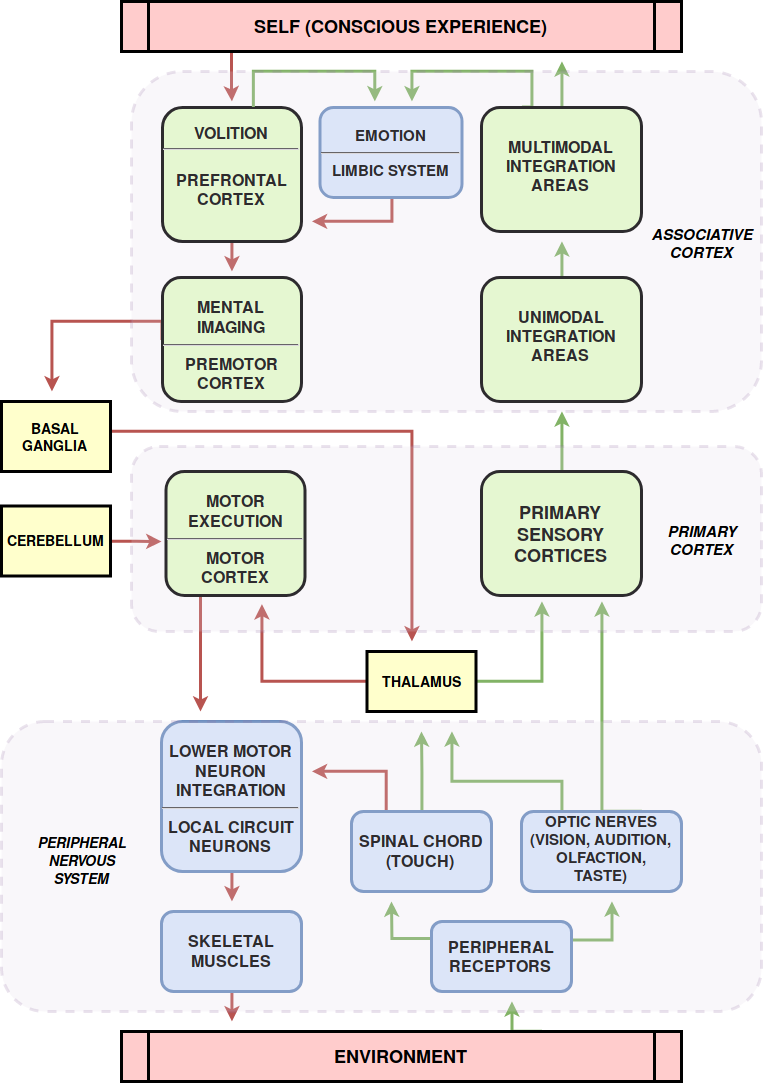
\includegraphics[width=.85\textwidth]{figures/brain_and_env.png}
   \end{figure}
  \end{column}
 \end{columns}
\end{frame}

\begin{frame}{Primary Areas}
 \begin{columns}[T]
  \begin{column}{.4\textwidth}
    \begin{itemize}
      \item \small Primary areas receive input directly from the thalamus
      \item \small Sensory areas receive high-dimensional data for each modality (vision, audition, etc.)
      \item \small The motor cortex conveys the already planned movement and sends it to the muscles
      \item \small Primary cortices have the better and most differentiated 6-layer laminar structure
    \end{itemize}
  \end{column}
  \begin{column}{.6\textwidth}
   \begin{figure}[H]
    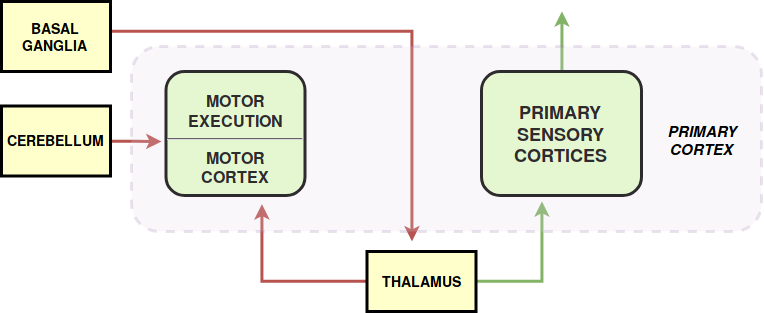
\includegraphics[width=1\textwidth, height=3.5cm]{figures/primary_structures.png}
   \end{figure}
   \vskip
   \begin{varblock}[7cm]{\scriptsize Olfaction is a special boy}
    \scriptsize Olfaction is the only sense that does not do thalamic relay in its
    path to the cortex. Signals from the nose go directly to the piriform cortex via the
    olfactory tract.
   \end{varblock}
  \end{column}
 \end{columns}
\end{frame}

\begin{frame}{Associative areas}

 \begin{columns}[T]
  \begin{column}{.4\textwidth}
    \begin{itemize}
      \item \small Can receive input from a diverse range of cortical areas
      \item \small As we go up on the hierarchy, it becomes ingreasingly difficult to pin down specific processes to brain regions
      \item \small There are two different sub-categories of associative areas: secondary (premotor cortex/unimodal integration areas) and tertiary (prefrontal cortex/multimodal integration)
    \end{itemize}
  \end{column}
  \begin{column}{.6\textwidth}
   \begin{figure}[H]
    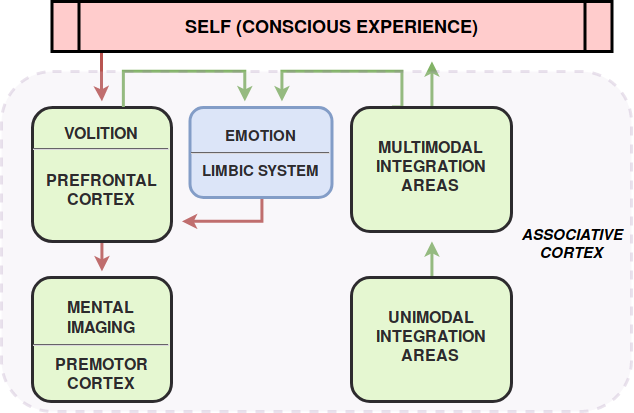
\includegraphics[width=.8\textwidth, height=3.5cm]{figures/associative_cortex.png}
    \end{figure}
   \vskip
   \begin{varblock}[7cm]{\scriptsize Neuroscientists do not agree on anyting - Part I}
    \scriptsize Although sometimes the term "associative" is used to designate all the cortex that is not a primary area, here we are referring only to sensory and motor association cortices.
   \end{varblock}
  \end{column}
 \end{columns}
\end{frame}

\begin{frame}{Secondary areas}

    \begin{itemize}
      \item They receive input mostly from their respective primary (sensory) or tertiary (motor) areas
      \item Secondary sensory areas show asymmetry patterns within each modality (more on that later)
      \item Secondary or premotor areas are mostly involved in the integration of all elements needed to perform movements
    \end{itemize}
    
\end{frame}

\begin{frame}{Tertiary areas}

    \begin{itemize}
      \item They constitute the link between higher cognition and their corresponding sensorimotor systems
      \item Information integrated from cognition that results in movement is feeded to secondary motor areas from tertiary motor areas, whereas tertiary sensory areas feed sensory representations to a variety of cortical areas
      \item The thalamus plays a crucial role in the widespread distribution both to and from these areas
      \item Processing in these areas does not involve perception or motor activities. Rather, they take charge of issue movements or integrate sensory representations across different sensory modalities
    \end{itemize}

\end{frame}

\section{The Motor System}

\begin{frame}{The Motor System: Function}

 \begin{columns}[T]
  \begin{column}{.5\textwidth}
  \vspace{.4cm}
    \begin{itemize}
      \item Unsurprisingly, it is in charge of controlling voluntary movements
      \item It is also in charge of controlling posture with the help of the vestibular system
      \item The primary motor cortex can be found anterior to the central sulcus. The premotor areas can be found anterior to the primary motor cortex. Both of them extend to the medial surface of the brain until the paracingulate sulcus
    \end{itemize}

  \end{column}
  \begin{column}{.6\textwidth}
   \begin{figure}[H]
   \vspace{-1.5cm}
    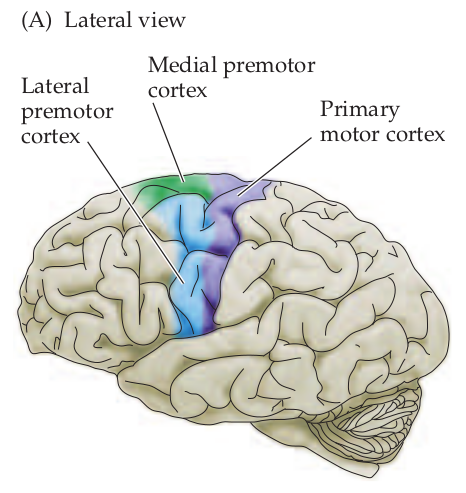
\includegraphics[width=.6\textwidth]{figures/motor_lateral.png}
   \end{figure}
   \vspace{-1cm}
   \begin{figure}[H]
    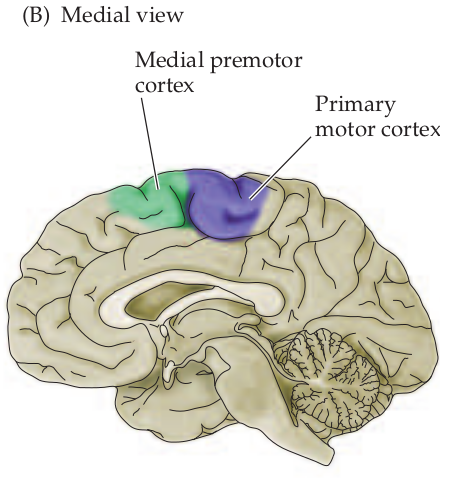
\includegraphics[width=.6\textwidth]{figures/motor_medial.png}
   \end{figure}
  \end{column}
 \end{columns}
    
\end{frame}

\begin{frame}{Primary Motor Cortex}

 \begin{columns}[T]
  \begin{column}{.5\textwidth}
   \vspace{.5cm}
    \begin{itemize}
      \item Follows a topographic organization of the body
      \item Each area contains populations of neurons specialized in movements rather than in innervating certain muscles
      \item The thalamus exerts a tonic inhibition on the motor system, and lifts this inhibition for areas where a movement is intended to be issued
    \end{itemize}

  \end{column}
  \begin{column}{.6\textwidth}
  \vspace{-1cm}
   \begin{figure}[H]
    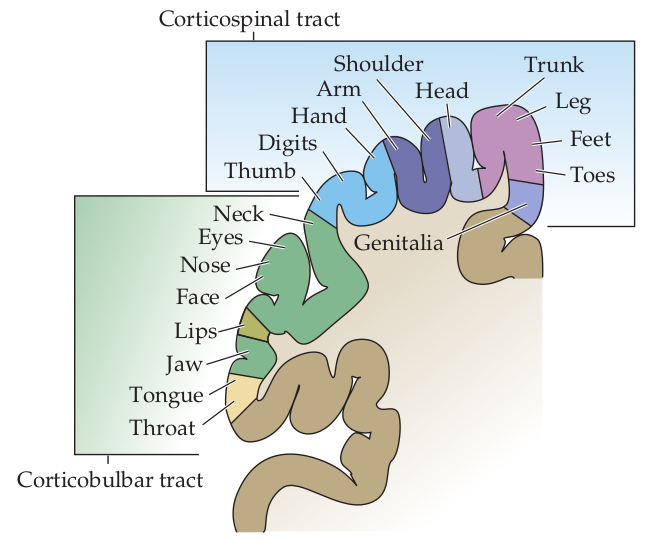
\includegraphics[width=.9\textwidth]{figures/primary_motor.png}
   \end{figure}
   
   \begin{varblock}[6.5cm]{\scriptsize Everything is crossed in the brain}
    \scriptsize As a rule of thumb, the brain processes information of the contralateral side of the body. Left hemisphere controls right side, and vice-versa
   \end{varblock}
  \end{column}
 \end{columns}
    
\end{frame}

\begin{frame}{Premotor Cortex}

    \begin{itemize}
      \item The premotor cortex uses information from other cortical areas to select movement appropiate to the context of the action
      \item The connections of this area are different when executing previously known moves in opposition to new moves
      \item In the case of new movements, they can be executed from observation or from memory, with different connections involved
   \end{itemize}
      
    \begin{varblock}[12cm]{Imagine your movements}
    If you "imagine" to move your arm, you can feel what it is like to activate this area of the brain witout ever reaching the actual motor cortex or muscles. This phenomenon applied to sports, music, and other areas is often called "mental play", and has shown strikingly effects in both profeesional musicians and sports players when used in addition to regular practice
    \end{varblock}

\end{frame}

\begin{frame}{Premotor Cortex}

    \begin{itemize}
      \item The medial premotor cortex has been shown to fire in pressence of the cue in learning experiments. It is linked to movement intention elicited by external elements
      \item On the contrary, medial premotor cortex has been shown to reflect the intention of movements
      elicited by internal elements
   \end{itemize}

\end{frame}
\end{document}
